\documentclass[xcolor=table]{beamer}


\usepackage[frenchb]{babel}

\usepackage[T1]{fontenc}

\usepackage[utf8]{inputenc}
\usepackage{amsmath}
\usepackage{graphicx}

\usetheme{default}

% \usetheme{Warsaw} -> A utiliser dans un second temps


\title[Automates]{Automates : quelques compléments}

\author{Jean-Christophe Le Lann}

\institute{ENSTA Bretagne}

\date{\today}


\begin{document}


\begin{frame}
\titlepage
\end{frame}

\begin{frame}{Rappels}
  L'Electronique numérique peut se définir comme la construction progressive de dispositifs complexes
  à partir d'élements simples :
  \begin{itemize}
    \item Eléments \textbf{combinatoires} : portes logiques de base (NOT,AND,OR etc voire seulement NAND ou NOR)
    \item Eléments \textbf{séquentiels} : bascules D et mémoires
  \end{itemize}
\end{frame}

\begin{frame}{Patterns de construction}
  Il existe un grand nombre de {\it patterns} de construction :
  \begin{center}
    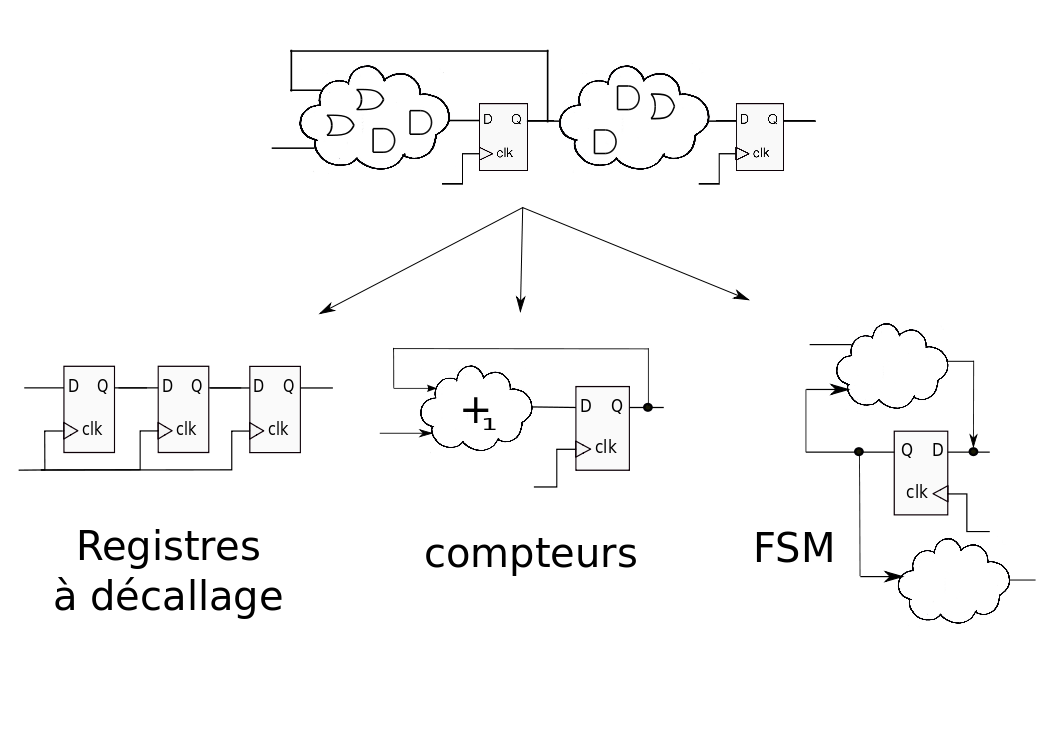
\includegraphics[width=6cm]{../../POLY/figures/synchrone.png}
  \end{center}

  Toutefois, pour l'Informaticien théoricien, ces éléments séquentiels se définissent tous comme des \textbf{automates}.

  Les \textbf{automates} ont donc une importance particulière dans le cadre étudié.

\end{frame}

\begin{frame}{Définition formelle d'un \textbf{automate de Moore}}
  Une automate de Moore est un sextuplet $(Q, \Sigma, \Delta, \sigma, \lambda, q_0 )$ :
  \begin{itemize}
  \item $Q$ est un ensemble fini d’états, $q_0$ est l’état initial
  \item $\Sigma$ est l’alphabet d’entrée, $\Delta$ est l’alphabet de sortie
  \item $\delta$ est une application de $Q \times \Sigma $ dans $Q$ : {\it fonction de transition}
  \item $\lambda$  est une application de $Q$ dans $\Delta$, donnant la sortie associée à chaque état
  \end{itemize}

  La sortie de l'automate de Moore en réponse à une entrée $a_1 a_2\dots a_n$ , $n \geq 0$ est
  $\lambda(q_0),\lambda(q_1)\dots \lambda(q_n)$ où
  $q_0 ,\dots, q_n$ est la séquence d’états tels que $\lambda(q_{i-1},a_i) = q_i$ pour $1 \leq i \leq n$.
  Remarque: Un automate de Moore retourne la sortie $\lambda(q_0)$ pour toute entrée.
\end{frame}

\begin{frame}{Définition formelle d'un \textbf{automate de Mealy}}
  Une automate de Mealy est un sextuplet $(Q, \Sigma, \Delta, \sigma, \lambda, q_0 )$ :
  \begin{itemize}
  \item $Q$ est un ensemble fini d’états, $q_0$ est l’état initial
  \item $\Sigma$ est l’alphabet d’entrée, $\Delta$ est l’alphabet de sortie
  \item $\delta$ est une application de $Q \times \Sigma $ dans $Q$ : {\it fonction de transition}
  \item $\lambda$  est une application de $Q\times \Sigma$ dans $\Delta$, donnant la sortie associée à chaque état
  \end{itemize}

  $\lambda(q, a)$ donne la sortie associée à une transition d’un état q sur l’entrée a.
  La sortie de l'automate de Mealy,en réponse à une séquence d’entrées $a_1,\dots a_n$ est
  $\lambda(q_0, a_1) \lambda(q_1 , a_2 ) \dots \lambda(q_{n-1}, a_n)$
  où $q_0 , q_1 ,\dots, q_n$ est la séquence des états tels que
  $\lambda(q_{i-1}, a_i) = q_i$ pour $1 \leq i \leq n$.
\end{frame}

\begin{frame}{Représentations proches de la réalisation électronique}
  \begin{figure}[h!]
    \centering
    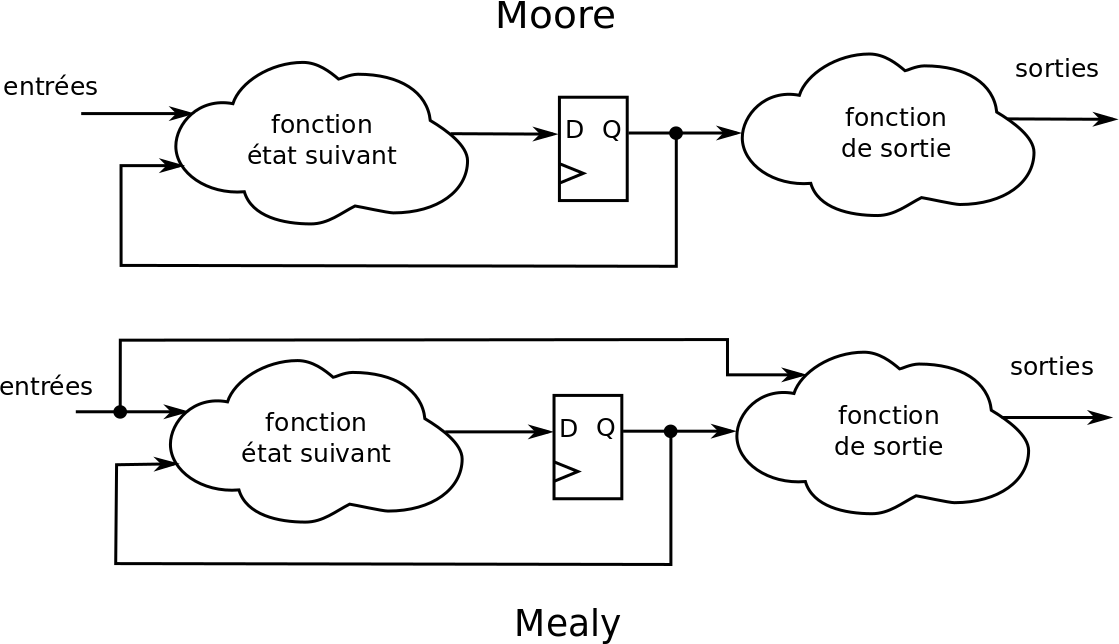
\includegraphics[scale=0.20]{../../POLY/figures/moore_mealy.png}
    \caption{Automates de Moore et de Mealy}
    \label{fig:mealy_moore}
  \end{figure}
\end{frame}

\begin{frame}{Concevoir un automate}
  Un problème de conception d'automate peut se résumer de la manière suivante :
  \begin{enumerate}
    \item Formulation du problème $\rightarrow$ diagramme états-transitions.
    \item Vérification de la {\it causalité} de l'automate décrit.
    \item Encodage des états.
    \item Construction du tableau de séquencement (si nécessaire)
    \item Détermination des fonctions d'état suivant (fonction de transition) et sorties.
  \end{enumerate}
  $$ D_i=f(Q_j,E_k) $$
  $$ S_l=g(Q_j,(E_k)) $$

  \begin{figure}[h!]
    \centering
    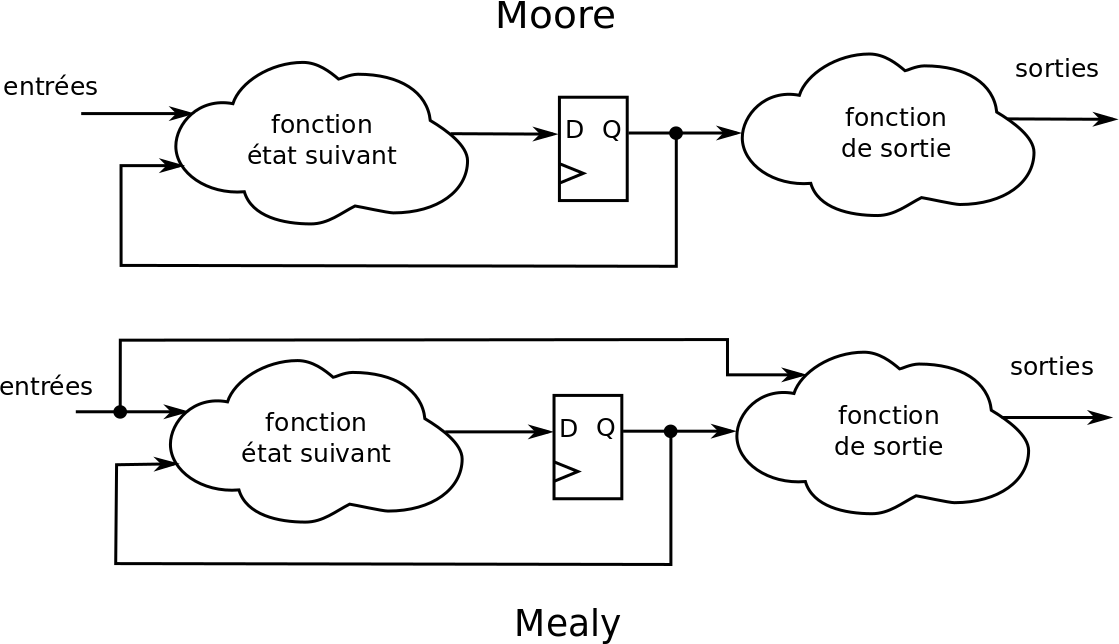
\includegraphics[scale=0.13]{../../POLY/figures/moore_mealy.png}
    %\caption{Automates de Moore et de Mealy}
    \label{fig:mealy_moore}
  \end{figure}
\end{frame}

\begin{frame}{Vérification de causalité d'automate}
  Pour qu'un automate soit considéré comme consistant ou {\it causal}, on doit examiner les conditions $c_i(s)$ des transitions
  partant de chaque état $s\in Q$.
  \begin{itemize}
  \item \textbf{Réactivité} Les conditions sur les transitions doivent être {\it collectivement exhaustives} : il existe forcément une transition à '1'.
  $$\forall s \in Q : \sum_i c_i(s)=1$$
  \item \textbf{Déterminisme} Les conditions sur les transitions doivent être {\it mutuellement exclusives} : on ne peut pas avoir deux transitions à '1' en même tem
  ps.
  $$\forall s \in Q, \forall (i,j), i\neq j : c_i(s).c_j(s)=0$$
  \end{itemize}
\end{frame}

\begin{frame}{Vérification de causalité d'automate (suite)}
  Cela signifie simplement que dans un état, il existe un, et un seul, état suivant.

  Notons qu'un état peut avoir comme état suivant lui-même : dans ce cas, le système décrit ne change pas d'état, tout simplement.
  En terme de diagramme états-transitions, cela revient à dessiner une boucle sur l'état (la "bulle").\\
\end{frame}

\begin{frame}{Etude de cas : vending machine (distributeur)}
  On cherche à réaliser un dispositif qui délivre un objet (cannette etc), après que l'on y a introduit 15 centimes.
  Ces 15 centimes peuvent être introduits à l'aide de pièces de 5 ou 10 centimes. La machine ne rend pas la monnaie.
  Concevoir cette machine.
\end{frame}

\begin{frame}{Etude de cas : diagramme états-transitions}
  \begin{figure}[h]
    \centering
    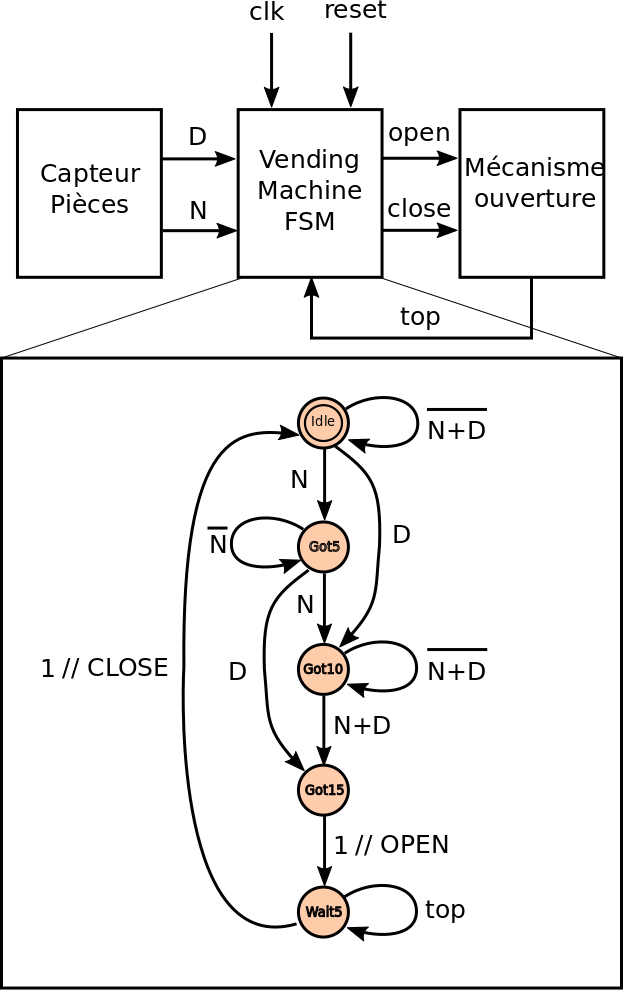
\includegraphics[scale=0.2]{../../POLY/figures/vending_machine.png}
    %\caption{Vending machine et son environnement}
    \label{fig:vending_machine}
  \end{figure}
\end{frame}

\begin{frame}{Etude de cas : encodage des états}
On rappelle que l'encodage des états consiste à associer un code binaire à chaque nom symbolique des états.
  \begin{itemize}
    \item Plusieurs encodages sont possibles.
    \item Chaque encodage conduit évidemment à des circuits différents structurellement, mais leur comportement
    aux entrées-sorties est identique.
    \item On retiendra deux encodages particuliers :
    \begin{enumerate}
      \item Encodage dense : numérotation binaire classique.
      \item Encodae "one-hot" : 1 bit par état. $1,2,4,8,16,32,...$
    \end{enumerate}
    \item L'encodage "one-hot" permet d'éviter les tableaux de Karnaugh.
  \end{itemize}
\end{frame}

\begin{frame}{Etude de cas : Encodage dense}

  \begin{minipage}{0.4\textwidth}

    \begin{figure}[h]
      \centering
      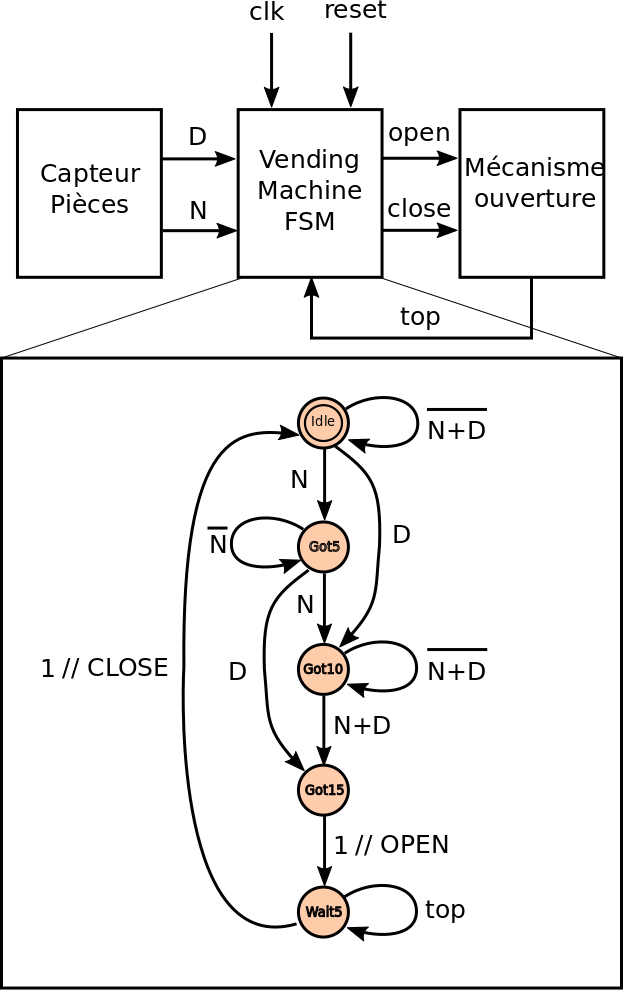
\includegraphics[scale=0.18]{../../POLY/figures/vending_machine.png}
      %\caption{Vending machine et son environnement}
      \label{fig:vending_machine}
    \end{figure}
  \end{minipage}
  \begin{minipage}{0.4\textwidth}
    \begin{table}
      \centering
      Encodage dense :
      \begin{tabular}{|l|c|c|}
            \hline
            état  & numéro & code binaire  \\ \hline \hline
            Idle  & 0      & 000           \\ \hline
            Got5  & 1      & 001           \\ \hline
            Got10 & 2      & 010           \\ \hline
            Got15 & 3      & 011           \\ \hline
            Wait5 & 4      & 100           \\ \hline
        \end{tabular}
    \end{table}
  \end{minipage}


\end{frame}

\begin{frame}{Etude de cas : encodage "one-hot"}
  \begin{minipage}{0.4\textwidth}

    \begin{figure}[h]
      \centering
      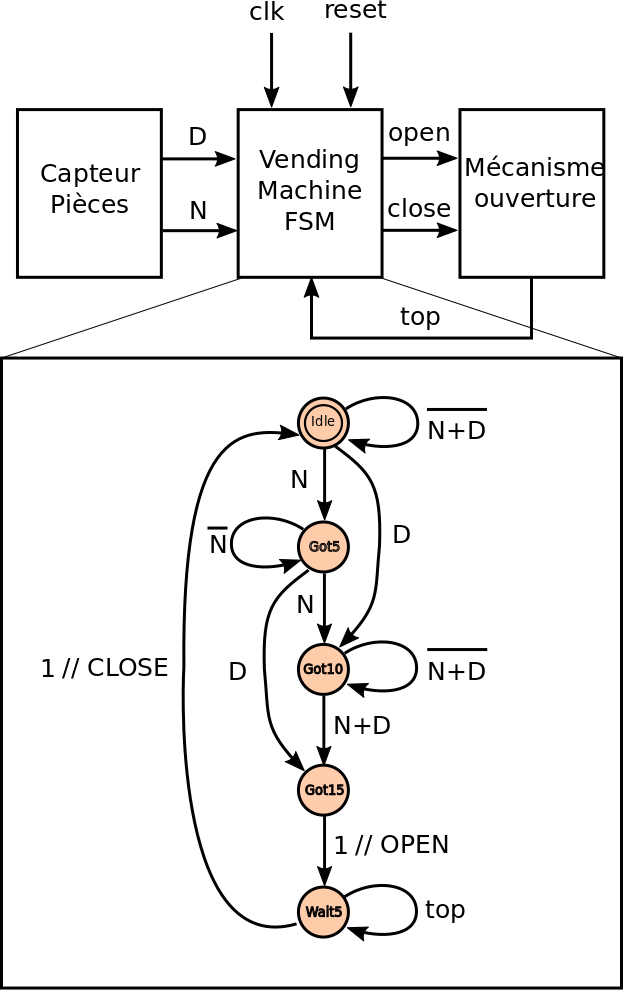
\includegraphics[scale=0.18]{../../POLY/figures/vending_machine.png}
      %\caption{Vending machine et son environnement}
      \label{fig:vending_machine}
    \end{figure}
  \end{minipage}
  \begin{minipage}{0.4\textwidth}
    \begin{table}[!htbp]
      \centering
      Encodage "one-hot" :
      \begin{tabular}{|l|c|c|}
            \hline
            état  & numéro & code binaire  \\ \hline \hline
            Idle  & 1       & 00001           \\ \hline
            Got5  & 2       & 00010           \\ \hline
            Got10 & 4       & 00100           \\ \hline
            Got15 & 8       & 01000           \\ \hline
            Wait5 & 16      & 10000           \\ \hline
        \end{tabular}
    \end{table}
  \end{minipage}
\end{frame}

\begin{frame}{Etude de cas : table de séquencement}
  Le but est de trouver les équations :   $$ D_i=f(Q_j,E_k) $$
    $$ S_l=g(Q_j,(E_k)) $$


Dans un premier temps on conserve les noms des états symboliques.
{\footnotesize
\begin{table}[!htb]
  \centering

  \begin{tabular}{|c|c|c|c||c|c|c|c|}
        \hline
        \cellcolor{blue!25} état courant & $e_1$ & ... & $e_n$ &  \cellcolor{red!25} état suivant & $s_1$ & ... & $s_n$ \\ \hline
        IDLE        & ~    & ~     & ~            & ~            & ~        & ~   & ~    \\ \hline
        \dots       & ~    & ~     & ~            & ~            & ~        & ~   & ~    \\ \hline
        GOT5        & ~    & ~     & ~            & ~            & ~        & ~   & ~    \\ \hline
        \dots       & ~    & ~     & ~            & ~            & ~        & ~   & ~    \\ \hline
    \end{tabular}
\end{table}
}

Puis on utilise l'encodage explicitant les $Q_i$ (état courant) et $D_i$ (état futur).
{\footnotesize
\begin{table}[!htb]
  \centering
    \begin{tabular}{|c|c|c|c|c|c||c|c|c|c|c|c|}
        \hline
        \cellcolor{blue!25}$Q_n$ & \cellcolor{blue!25}\dots & \cellcolor{blue!25} $Q_0$ &  $e_1$ & ... & $e_n$ & \cellcolor{red!25}$D_1$ & \cellcolor{red!25}\dots & \cellcolor{red!25}$D_0$ & $s_1$ & ... & $s_n$ \\ \hline
        ~   & ~    & ~  & ~  & ~  & ~  & ~  & ~  & ~        & ~   & ~ & ~        \\
        ~   & ~    & ~  & ~  & ~  & ~  & ~  & ~  & ~        & ~   & ~ & ~        \\
        \hline
    \end{tabular}
\end{table}
}

\end{frame}

\begin{frame}{Etude de cas : équations finales}
Il reste à observer les colonnes des $D_i$ et $s_j$ et déduire les équations logiques
  \begin{itemize}
    \item Déduction immédiate dans certains cas.
    \item Construction des tableaux de Karnaugh pour chaque $D_i$ et $s_j$
  \end{itemize}
\end{frame}


\begin{frame}{Cas de l'encodage One-Hot}

  On peut {\it bypasser} les étapes précédentes dans le cas d'un automate dont les états sont encodés One-Hot, et déduire
  les équations par simple observation du diagramme états-transitions et application du schéma de traduction suivant :


  \begin{figure}[!htp]
    \centering
    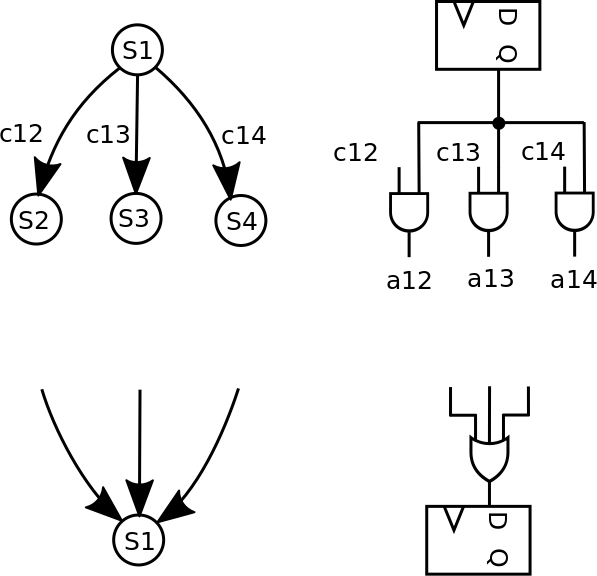
\includegraphics[scale=0.2]{../../POLY/figures/one_hot_method.png}
    %\caption{Procédé simplifiant la génération d'un circuit d'automate dans le cas d'un encodage {\it one-hot}.}
    \label{fig:one_hot}
  \end{figure}
\end{frame}

\begin{frame}{Cas de l'encodage One-Hot}

  \begin{itemize}
    \item On dessine une bascule $D$ pour un état $S$
    \item Pour chacune des transitions sortantes d'un état $S_i$ vers un état $S_j$, on dessine une porte AND connectée d'une part à la sortie $Q$ de la bascule de l'état $S_i$, et
    d'autre part la condition booléenne $c$ de la transition $S_i\rightarrow_{c} S_j$. Appelons $c_{i,j}$ la sortie de cette porte AND.
    \item Pour chacune des transitions entrantes d'un état $S_j$ on dessine une porte OR connectée à l'entrée $D_j$ et possédant autant d'entrées qu'il existe de transitions entrantes.
    A partir des états précedents $S_i$, on connecte le signal $c_{i,j}$ sur une des entrées de cette porte OR.
  \end{itemize}

\end{frame}


\begin{frame}{Dessin du circuit}
Dans certains cas simples, il reste possible de dessiner le circuit. Sinon, on s'en tient
au schéma d'ensemble suivant :

\begin{figure}[!htp]
  \centering
  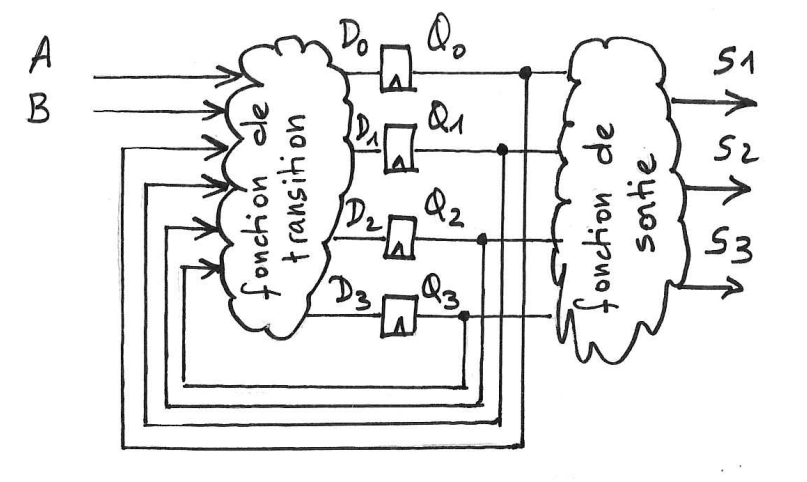
\includegraphics[scale=0.2]{./circuit_template.png}
  %\caption{Procédé simplifiant la génération d'un circuit d'automate dans le cas d'un encodage {\it one-hot}.}
  %\label{fig:one_hot}
\end{figure}

\end{frame}

\end{document}
